%update: Dec 13 figures added, references pending...
%update: Nov 21 first copy draft

\begin{savequote}[75mm] 
You may say I'm a dreamer, but I'm not the only one. I hope someday you'll join us. And the world will live as one.
\qauthor{John Lennon} 
\end{savequote}

\chapter{Opto-mechano-electrical tripling in ZnO nanowires probed by \emph{In situ} photocurrent spectroscopy in TEM}

\newthought{To find clues} for flexible optoelectronics, light, force and electrons are all important factors to be considered. Photocurrent spectroscopy of individual free-standing ZnO nanowires inside a high-resolution transmission electron microscope (TEM) is reported. By using specially designed optical in situ TEM system capable of scanning tunneling microscopy (STM) probing paired with light illumination, opto-mechano-electrical tripling phenomenon in ZnO nanowires is demonstrated. Splitting of photocurrent spectra at around 3.3 eV under {\em in situ} TEM bending of ZnO nanowires directly corresponds to nanowire deformation and appearance of expanded and compressed nanowire sides. Theoretical simulation of a bent ZnO nanowire has an excellent agreement with the experimental data. The splitting effect could be explained by a change in the valence band structure of ZnO nanowires due to a lattice strain. The strain-induced splitting provides important clues for future flexible piezo-phototronics. 

\section{Introduction}

The current and future progress in transferring large blocks of information at ultra-high speed with marginally low power consumption relies on using photons in optical waveguides instead of electrons in copper wires. However, the social communities are still not completely satisfied with rather small capacities, low speeds, high power consumption and high complexity in integrations of information transfer pathways on rigid or flexible substrates.\cite{C.2009, T.2004, D.2004}
To achieve effective integrations with multi-functionalities, the sizes of light sources for modulators, resonators, light guides, photo-detectors, strain sensors and accelerometers etc. in Micro-Opto-Electro-Mechanical Systems (MOEMS) are expected to reach hundreds of nanometers.\cite{E.2007} However, decreasing size does straightforwardly lead to the optoelectronic device performance enhancement. To catch up with the presently well-established electronics the light-matter interactions should be thoroughly studied and understood both by theoretical simulations and experiments due to the key difference between electrons and photons; the latter exhibit wavelengths down to hundreds of nanometers (UV-visible) and up to ~ 1550 nm (the range which is widely used in fiber communication technologies). However, conventional approaches can hardly detect, operate and modify optoelectronic behaviors of a nanomaterial in real time and at high spatial resolution. 

\begin{figure}  
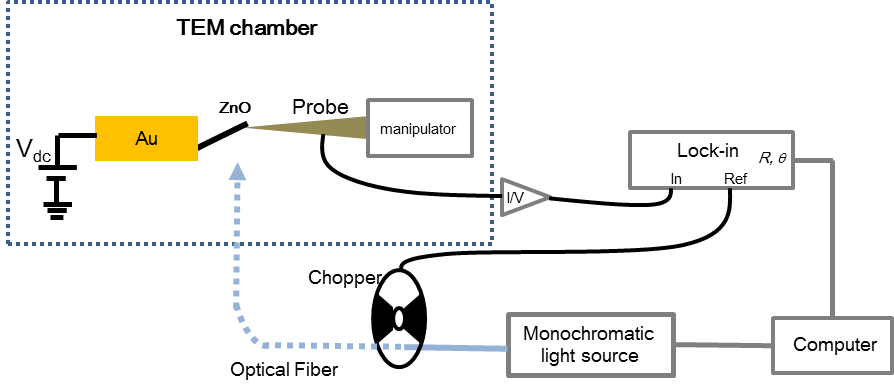
\includegraphics[width=\textwidth]{figures/figure5_1}
\caption[Experimental setup for ZnO.]{Scheme of experimental configuration inside and outside of a high-resolution TEM.
\label{fig:5_1}}
\end{figure}

Moreover, flexible and stretchable optoelectronics attracts general attentions in recent years. Nanowire, as one of scientists’ favorite building blocks for flexible optoelectronics has not been yet carefully studied as a single free-standing physical object. Zinc oxide (ZnO) nanowire is one of the most promising materials for opto-mechano-electrical applications due to its excellent piezo-phototronic properties.\cite{L.2011a,L.2010,D.2015,L.2010a} However, previous reports on flexible nanowire photodiode detectors were performed on materials placed on substrates.\cite{G.2015,H.2014,G.2014} Clearly, choosing a proper substrate is always an essential step in flexible optoelectronics; hence the physical behaviors of a nanostructure are strongly influenced by substrates and spacious metal electrodes. For example, it has been found that the optical absorption coefficient, the band-edge and near-band-edge (NBE) characteristics of ZnO films are all dependent on the substrate quality and subsequent treatments.\cite{R.1997} Therefore, it is essential to characterize mechano-optoelectronic properties of ZnO nanostructures in a free-standing configuration and in high vacuum. For example, Ohno et al. studied photoluminescence and cathodoluminescence (CL) spectra of a diamond crystal in TEM;\cite{S.1995} Yang et al. measured photocurrent values of bent ZnO nanowires in TEM under fixed wavelength light.\cite{E.2012} However, the wide-band-range photocurrent spectroscopy of ZnO nanowires (or any other nanomaterial) has not been studied as yet. 
Herein we report on the photocurrent spectroscopy of individual free-standing ZnO nanowires by means of a special optical-STM-TEM system. It is found that the photocurrent spectra of ZnO nanowires experience a specific splitting, and the shift values perfectly correlate with the bending strains. Under relevant theoretical simulations, the valence band structure was found to change accordingly. The simulations fitted and confirmed the experimental results. 

\section{Experimental}

ZnO nanowires were synthesized by a chemical vapor deposition (CVD) method, as was reported in detail previously.\cite{D.2015} In situ characterizations and manipulations were carried out by an optimized {\em Nanofactory Instruments AB} opto-TEM-STM sample holder with a nanomanipulator and an optical fiber in a 300 kV JEOL-3100FEF (Omega filter) high-resolution microscope. An optical fiber thread inside the side entry holder was connected to the optical system outside of the TEM column. ZnO nanowires were securely attached onto the gold wire stage within the holder tip-frame by using a silver paste. Then, inside TEM, the electrochemically etched sharp tungsten probe was manipulated to contact a pre-selected individual nanowire using the piezo-nanomanipulator, while at the same time, the movable optical fiber was aligned to illuminate the nanowire with a light accordingly. The experimental configuration is schematically shown in Figure \ref{fig:5_1}. By manipulating the tungsten probe, bending of nanowires was precisely controlled. The photocurrent was measured by applying a bias between the two ends of a ZnO nanowire which was directly illuminated by light at a certain wavelength. As a monochromator scanned from 2.5 eV to 4.5 eV, a spectrum of photocurrent vs photon energy could be obtained. Then, by using a lock-in amplifier, photocurrent signal could be rectified according to chopper frequency. 

\begin{figure}  
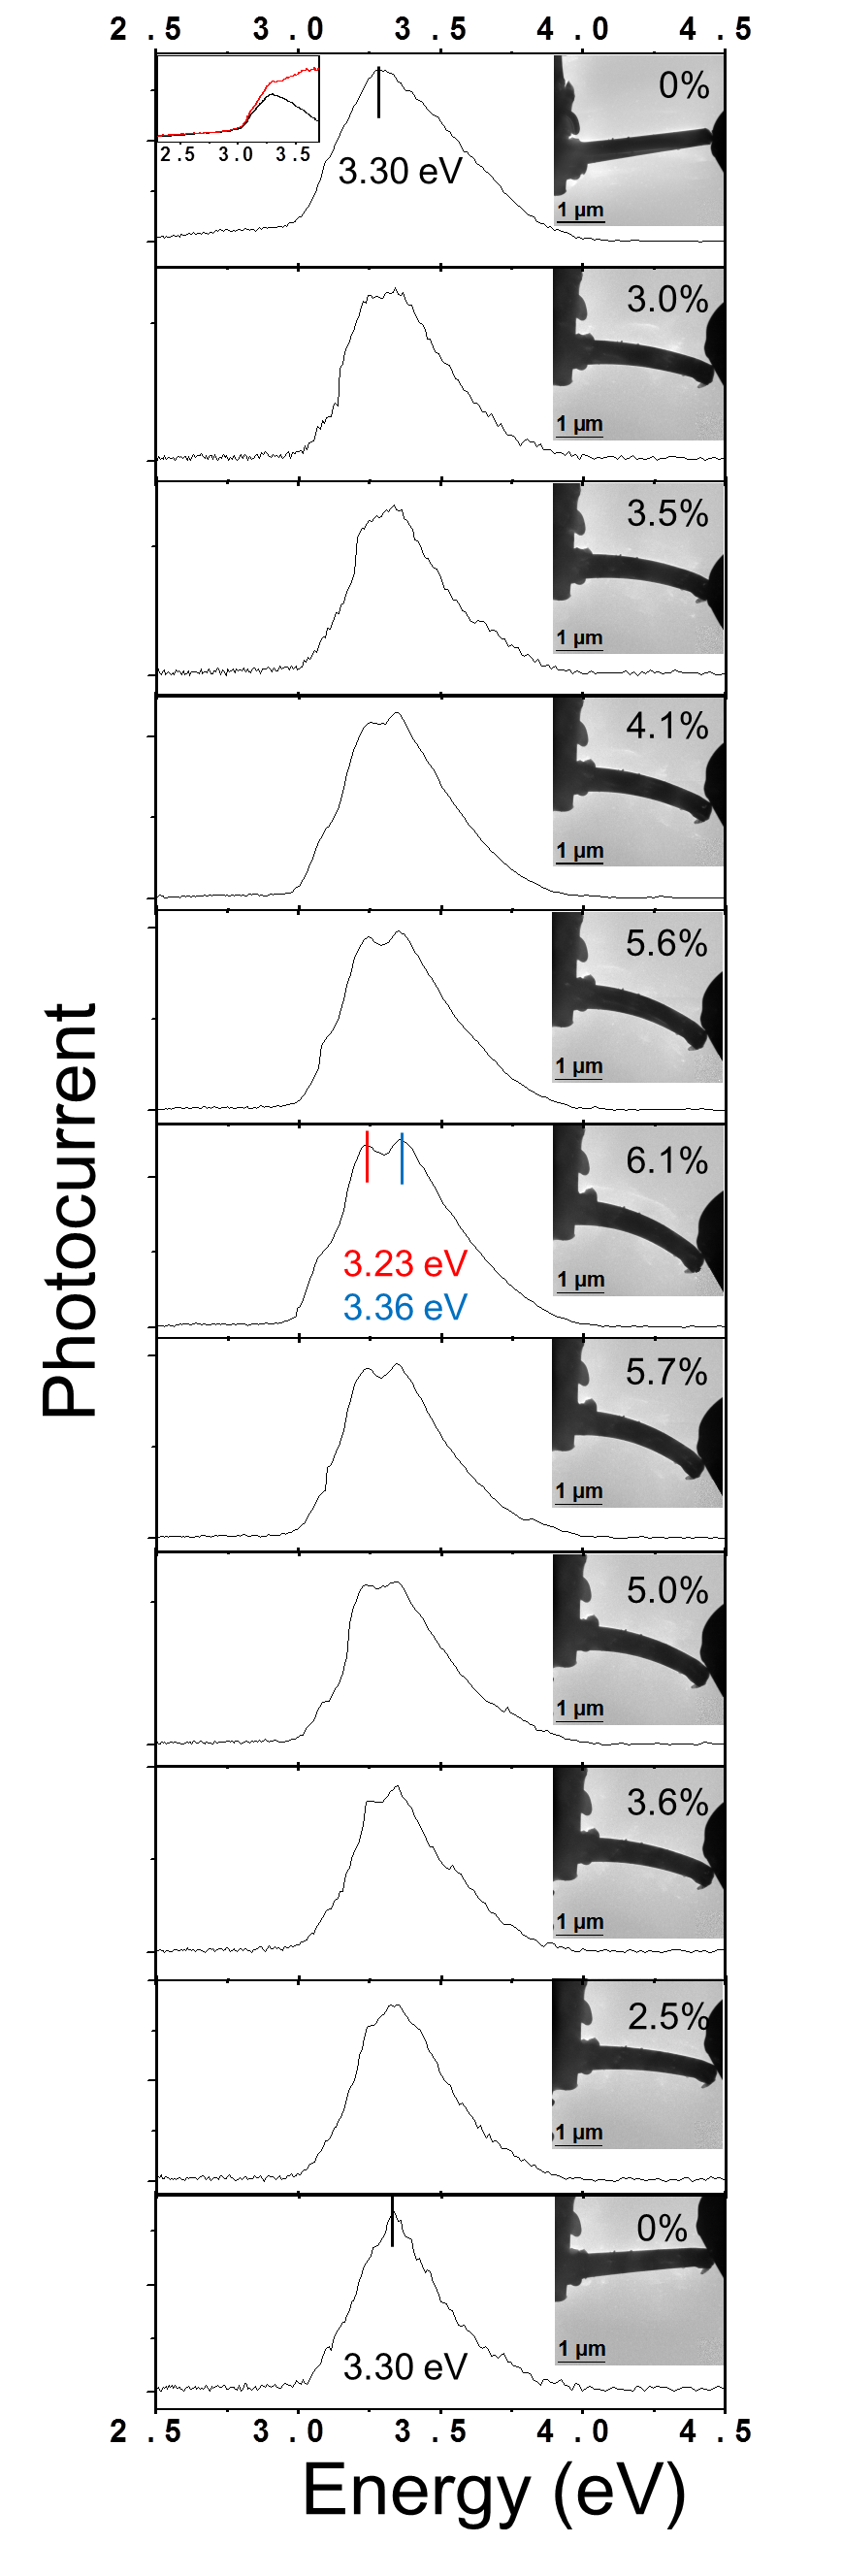
\includegraphics[width=150pt]{figures/figure5_2}
\centering
\caption[Splitting of photocurrent spectroscopy.]{Photocurrent spectra (raw data) measured under bending deformations from 0\% to 6.1\%, and back to 0\%. Red line in the upper left inset of the first panel shows the normalized (to the incident photons) spectrum at the zero strain state (normalized from the measured photocurrents shown as the black line in the inset).
\label{fig:5_2}}
\end{figure}

\section{Results and disscussions}

In Figure \ref{fig:5_2}, a typical experiment on a representative ZnO nanowire is demonstrated. The nanowire was originally straight, as shown in the first panel of Figure \ref{fig:5_2}. The normalized (to the incident photons) spectrum at the zero strain state is displayed in the inset. Due to the large exciton binding energy of ZnO (~60 meV), even at room temperature, a clear exciton absorption peak was observed. By manipulating the probe, the nanowire was forced to bend in the horizontal plane. Photocurrent-wavelength raw data curves in Figure \ref{fig:5_2} demonstrate the regarded splitting phenomenon during photocurrent spectroscopy, which is related to the strain in the bent nanowire. The diameter of the nanowire is 385 nm. The bending ratio, or strain, was determined as follows: $$\epsilon = \frac{r}{R} $$
, where $r$ is a distance from the compressed/expanded side of the nanowire to the middle point of the compressed/expanded region, respectively, $R$ is a radius of curvature of the nanowire. The first manipulation bent the nanowire to a 3.0\% strain, and then gradually to 3.5\%, 4.1\%, 5.55\% and 6.1\%. Finally, the probe was carefully moved backwards, while the strains decreased to 5.66\%, 5.0\%, 3.6\%, 2.5\%, finally giving the initial straight configuration. Before taking a photocurrent spectrum after each manipulation, the electron beam of the microscope was taken off and away from the sample. The inner side of the bent nanowire carries a compressive strain, and its outer side suffers an expansion. The high-resolution image (Figure \ref{fig:5_s2}) clearly demonstrates the nanowire (002) lattice fringes alone c-axis (growth direction) under strain.\cite{zhang2015opto} The lattice distance within the compressed nanowire edge is 0.243 nm, which is smaller than the usual value of 0.260 nm.\cite{L.2011} The lattice distance becomes gradually larger, away from the compressed edge, up to 0.257 nm. Upon bending, the photocurrent spectra first remain of the similar shape with one broad peak centered at around 3.30 eV. However, once the strain increases further, the originally broad peak splits into two fractions. Under a 3.0\% strain, these two peaks are centered at 3.24 eV and 3.34 eV. Thus the detected red-shift and blue-shift are 0.06 eV and 0.04 eV, respectively. Under the largest strain utilized, 6.1\%, the red-shift increases to about 0.07 eV, and the blue shift to 0.06 eV. The splitting values (the gap between the two peaks) of photocurrent spectra of the bent nanowire were 0.01 eV (3.0\%), 0.09 eV (3.5\%), 0.10 eV (4.1\%), 0.12 eV (5.6\%), 0.13 eV (6.1\%), 0.11 eV (5.7\%), 0.13 eV (5.0\%), 0.10 eV (3.6\%) and 0.08 eV (2.5\%), in sequence. The peak positions are displayed in Figure \ref{fig:5_3}(d) to show the relationship with strain values. It is obvious that there is a clear correlation between the strain and peak position shifts. To better understand such correlation, a theoretical simulation was performed. Measuring photocurrent spectrum is one of the methods to obtain the band gap information. Therefore the researchers typically explain photocurrent phenomena by band gap theories. In our work, ZnO nanowire is a well-structured direct band gap material tested without a substrate and in high vacuum conditions peculiar to a high-resolution TEM. Therefore, it is currently reasonable to assume that changing of the band gap is directly connected with the corresponding energy values of the photocurrent peak and its splitting. Because the contribution of splitting is not the prime one with respect to the overall spectrum broadening, and the total spectra contain a photoresponse affected by some pre-existing defects (not created by bending), the spectrum broadening due to splitting is probably hidden. Another fact is that the fiber efficiency used in our measurement system is rather limited. The transmission efficiency descends significantly at the UV range, at around 400 nm (~ 3.1 eV), this cuts off the intensity of the incident light energy. 

\begin{figure}  
\centering
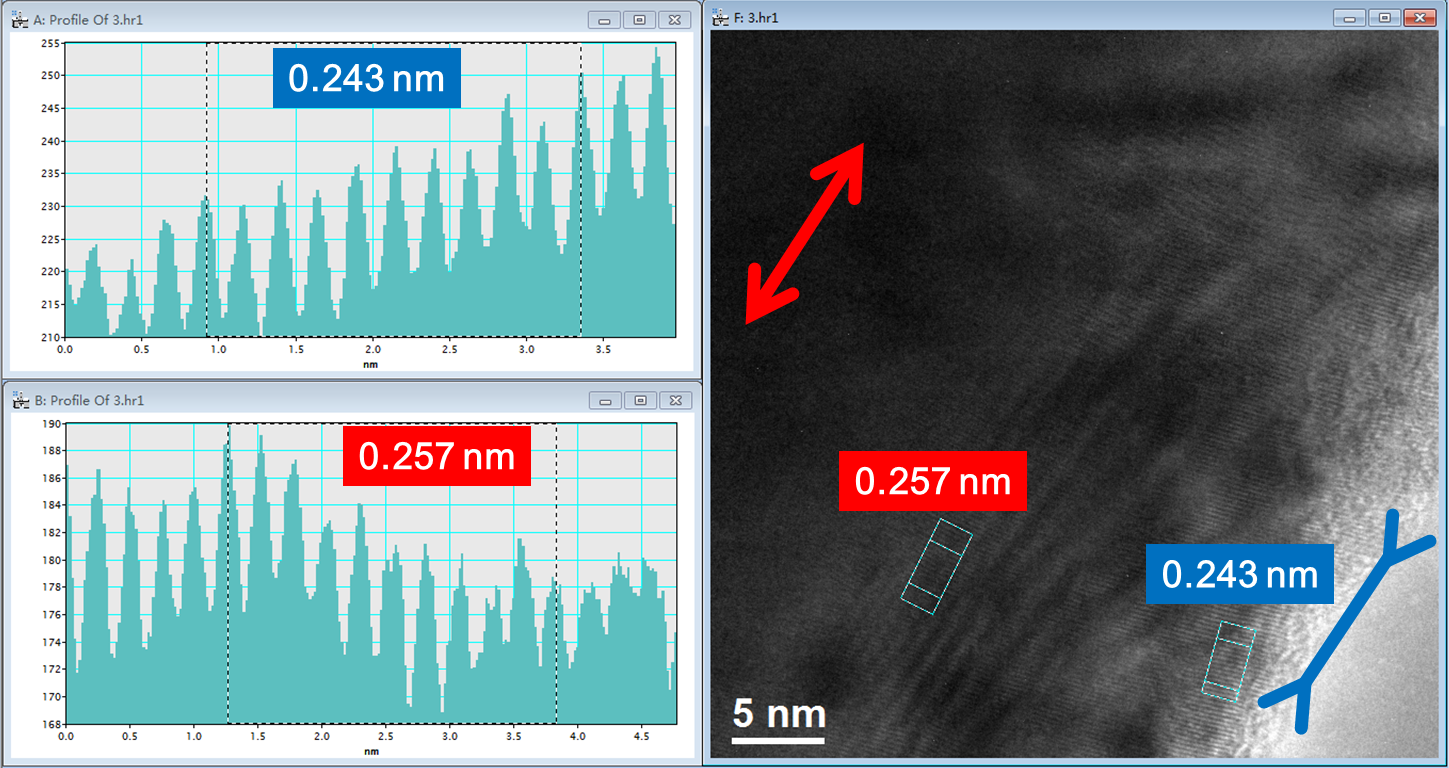
\includegraphics[width=\textwidth]{figures/figure5_s2}
\caption[Localized strain in HRTEM image]{High-resolution TEM image of a bent ZnO nanowire. The (002) lattice fringe separation is 0.243 nm at the very compressed sample edge, and 0.257 nm at the less compressed core. 
\label{fig:5_s2}}
\end{figure}


Theoretical simulation of bent ZnO nanowires was carried out using Density Functional Tight Binding (DFTB) method, implemented in DFTB+ software package.\cite{T.2007} DFTB approach has widely been used for the accurate description of structural, electronic and transport properties of various compounds which contain a large number of atoms in the unit cell (more than 1000). However, because of calculation capability limitations with respect to the number of atoms involved, we simulated a ZnO nanowire with diameter of ~1.5 nm. Parameterization of Zn atom interactions with O atoms has been tested for many bulk Zn-based solids (hcp-Zn, zinc-blende-ZnS and wurtzite-ZnO), ZnO surfaces (clean and with a small amount of adsorbates), and ZnO nanostructures. Such parameterization has provided a reliable description of electronic band structures of ZnO, including reasonable representations of the valence and conduction bands and a band gap of ~ 4.1 eV.\cite{T.2009}

\begin{figure}  
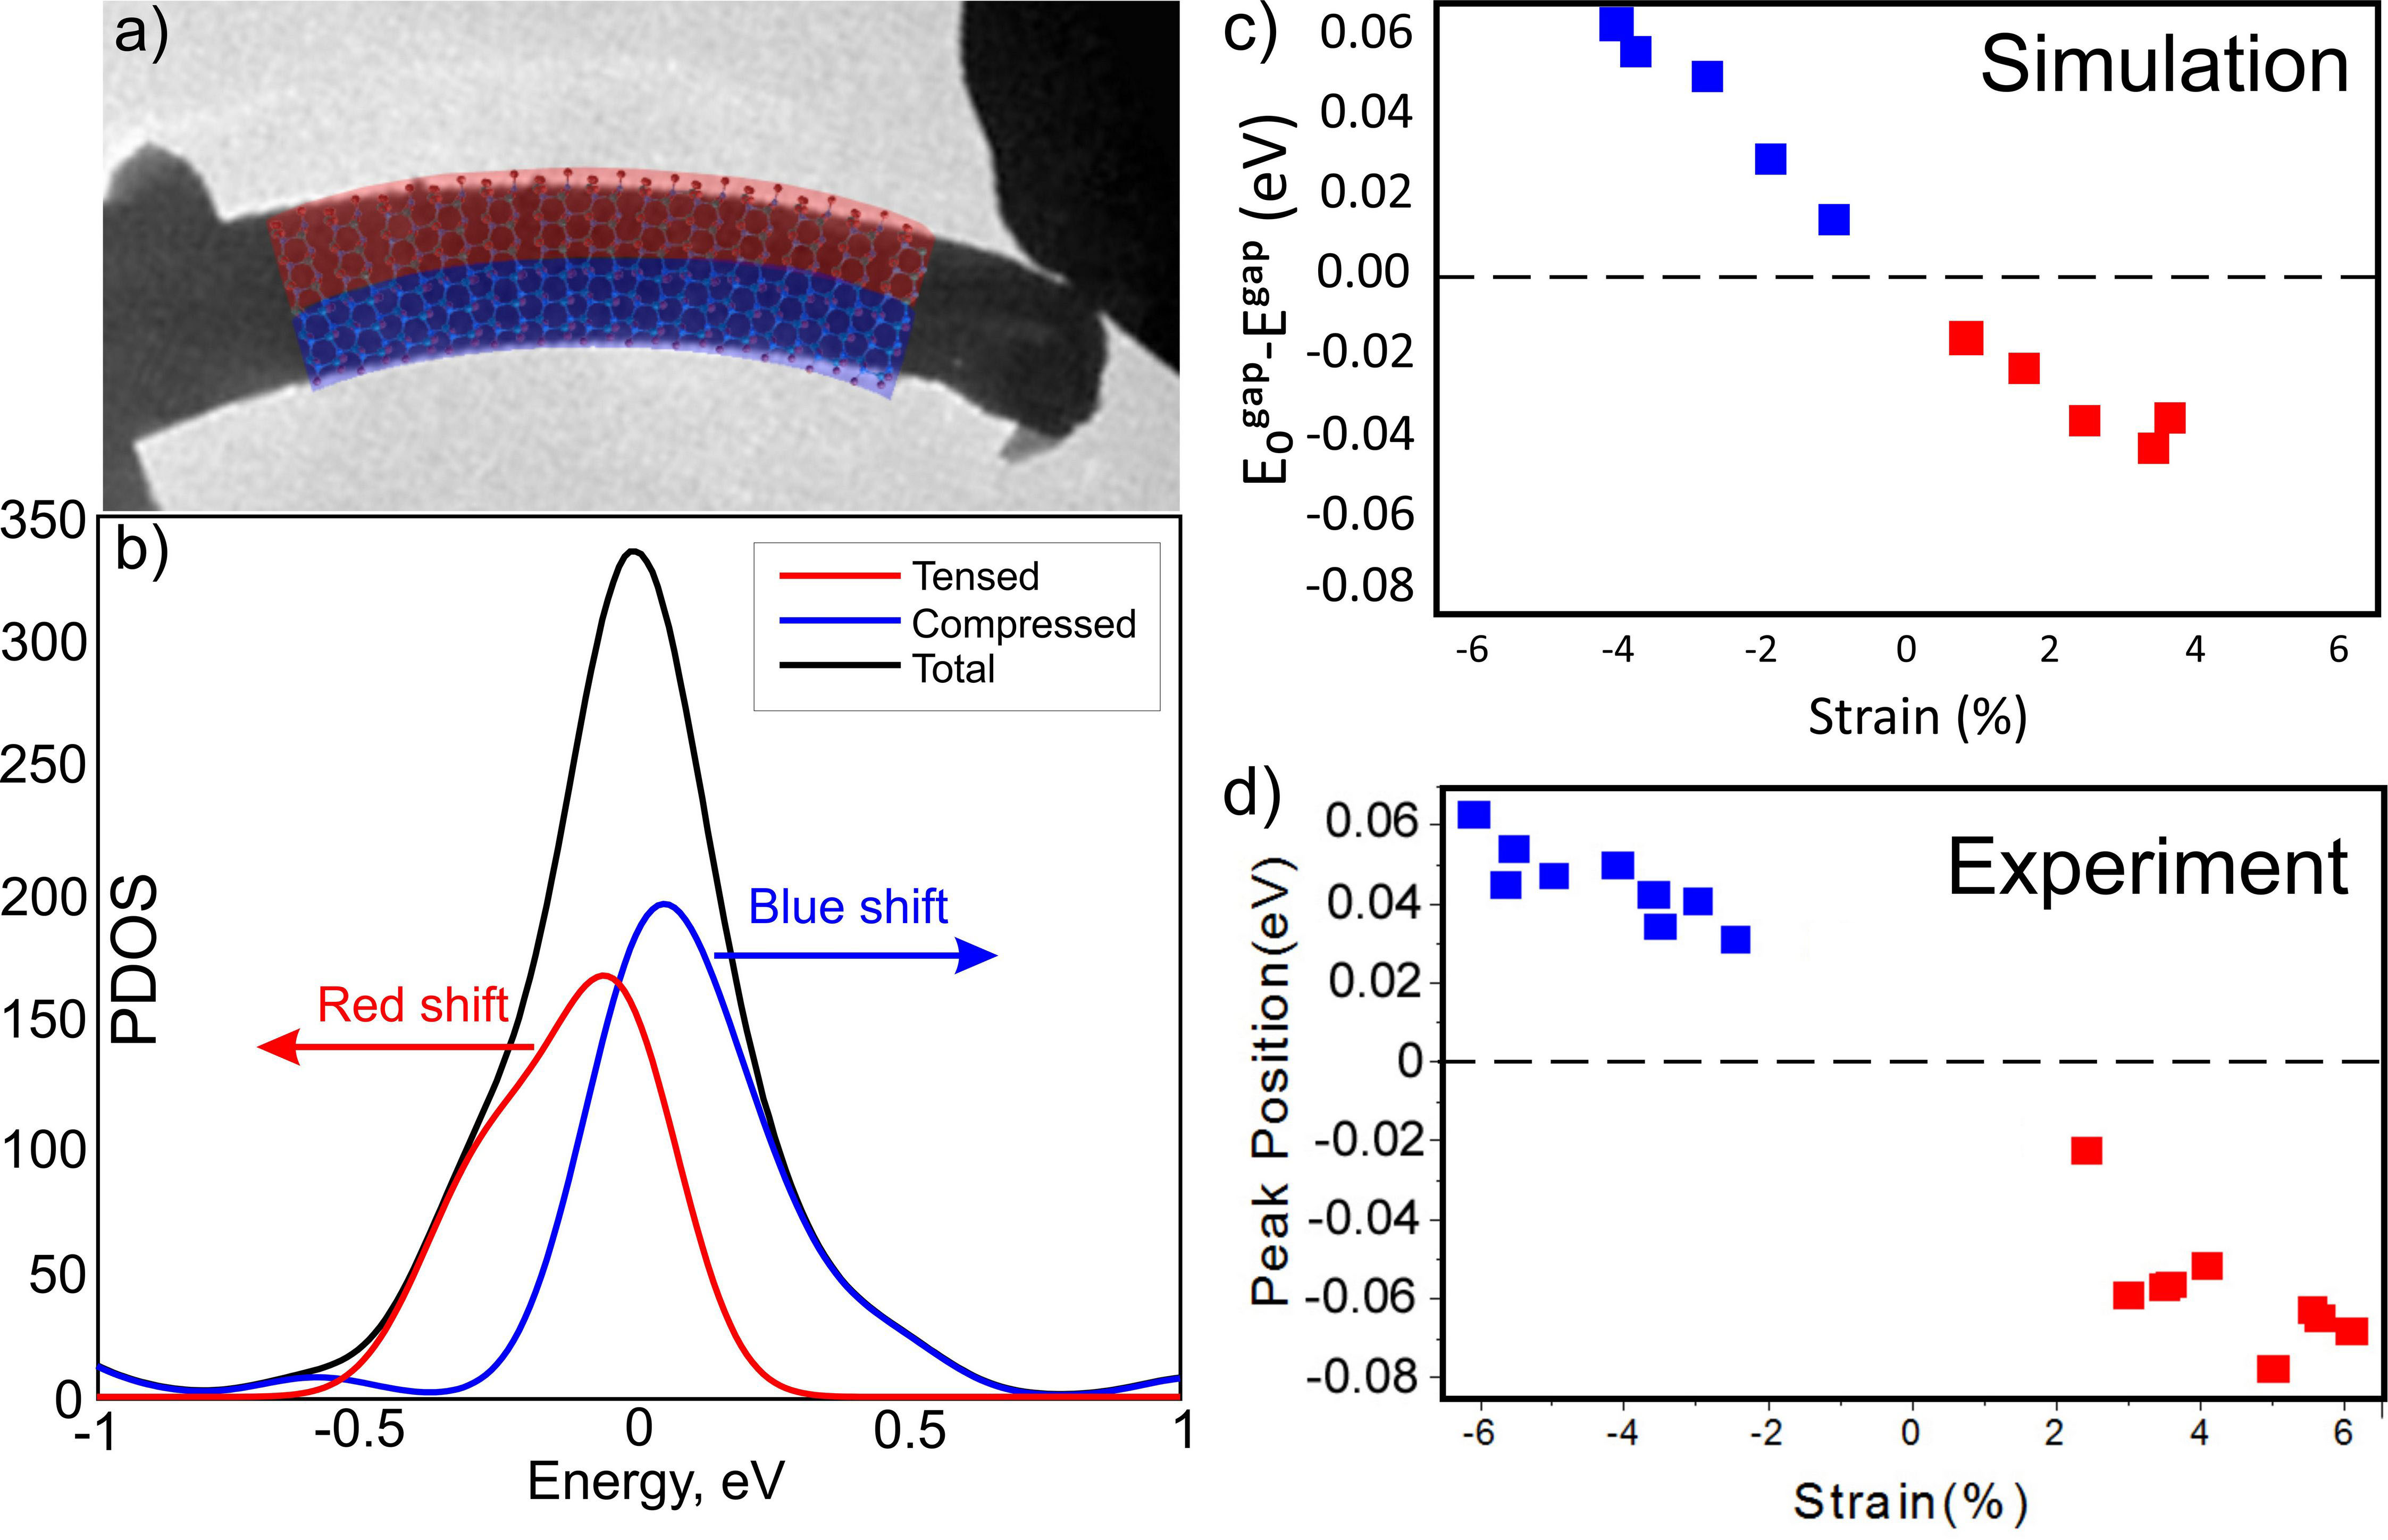
\includegraphics[width=\textwidth]{figures/figure5_3}
\caption[DFTB simulation match experimental result]{(a) Simulated geometry of a bent ZnO nanowire in comparison with the experimental picture. The simulated structure is divided into two parts (marked by red and blue regions) for the calculation of PDOS in expanded and compressed regions. Note that the size of simulation geometry is not the same as for the experimental image. (b) PDOS of expanded (red) and compressed (blue) sides of the deformed ZnO nanowire. Black curve denotes the total DOS for the undeformed nanowire as a whole. Bending strain is about 4\%. (c) Dependence of the ZnO wire band gap on the bending deformation in the frame of the DFTB approach utilized; (d) Dependence of the photocurrent peak position on the bending strain obtained experimentally. Red and blue colors correspond to the expanded and compressed regions of ZnO nanowires, respectively. 
\label{fig:5_3}}
\end{figure}


In the present modeling we simulated bent ZnO nanowires with various degrees of curvature in accord with the experimental deformation values, as shown Figure \ref{fig:5_3}(a). Two sides of the nanowire are marked in red color (expanded side) and blue color (compressive side), respectively. A simulated supercell of ZnO nanowire consisted of 1500 atoms of Zn and O. To avoid the presence of dangling bonds and surface currents over the bent nanowires they were covered by a uniform layer of hydrogen atoms. 
Splitting of the photocurrent peak directly corresponds to the splitting of levels in the valence band at $\Gamma$ point with the corresponding red and blue shifts of the peaked wavelength values under deformation.\cite{D.-P.2012} To calculate the values of splitting partial density of states (PDOS) was computed for the expanded and compressed sides of a nanowire, which is shown in Figure \ref{fig:5_3}(b). During bending, the position of conductive band was not changed; only changes of the valence band were distinguished. In Figure \ref{fig:5_3}(b), the changes in the valence band of the bent ZnO nanowire (having a bending deformation of about 4\%) are presented. PDOS peculiar to the expanded and compressed sides of the ZnO nanowire are depicted in red and blue colors, respectively. Simulation result confirmed that the valence band shifts in a direction of red range of wavelengths, whereas the compression leads to the blue shift, thus in a perfect match with the experimental data. The same calculations were then carried out for ZnO nanowires having various bending deformations (1-4\%). In Figure \ref{fig:5_3}(c) theoretically obtained dependence of the band gap on the bending ratio is shown. The changes in the band gap are directly correlated with the changes in the photocurrent peak positions measured in the experiments, as shown in Figure \ref{fig:5_3}(d). Thus the obtained computation results have an excellent agreement with the experimental data. 
A few reports in regards of bent ZnO nanowires/microwires support our results. Xue et al. probed the strain effects on NBE characterized by CL while studying a curved ZnO nanowire inside a scanning electron microscope (SEM) and found that the emissions had had a relation with the strain ratio.24 Liao et al. also studied CL splitting and shift in bent ZnO microwires in SEM; the authors documented the correlation between the excitation spectra evolution and compressive edges. And it was believed that the valence band splitting had contributed to NBE splitting.\cite{T.2009} In our experiments, the splitting takes place not during CL measurements, which is a process caused by an electron beam to emit light, but during recording of a photocurrent, which is a result of light absorption and electron-hole pairs’ generation. However, both processes share the same deformation conditions which cause the splitting of levels in the valence band at Г point. 


\section{Conclusions}
To sum up, this is a report on opto-mechano-electrical tripling phenomenon under in situ observation and measurements of photocurrents in ZnO nanowires in real time and under the highest spatial resolution natural for a high-resolution TEM instrument. By comparing nicely resolved photocurrent spectra of individual ZnO nanowires under bending deformations splitting of photocurrent spectra is observed. The shifts of photocurrent peaks are directly dependent on the bending strains. The red and blue shifts of ZnO photocurrent peaks under bending are confirmed to be directly related to the splitting of levels in the valence band at $\Gamma$ point. DFTB simulations have an excellent agreement with the experimental data. The discovered splitting effect under specially designed ZnO nanowire photocurrent spectroscopy provides an important information for flexible optoelectronics and piezo-phototronics, for example, for strain tuned wavelength-division multiplexing and MOEMS devices, and for flexible optoelectronics where photocurrent splitting should be evaded. 



